\chapter{Introduction}

Anomalies arise in many application fields, including cyber--security,
medicine or finance and their detection is sometimes crucial for understanding
new processes or mitigation of unwanted phenomena. A typical example
of the first case is an anomalous behaviour in a particle accelerator
which leads the physicists to carefully go through their data and
theories and return with the discovery of a new particle, while a
fraudulent credit card transaction is an example of the latter. With
the increasing volumes of collected data and processing power, automatic
detection of anomalies is as relevant as ever.

The terms outlier and anomaly are sometimes used interchangeably,
but in this text we will resort to the use of the second term. There
is no mathematical definition of what an anomaly is. The way that
other authors define what is an anomaly is usually in the spirit of
``an observation which deviates so much from other observations as
to arouse suspicion that it was generated by a different mechanism''~\cite{barnett1974outliers}.

There are countless models and algorithms for anomaly detection, tackling
the problem from different angles based on the basic principle of
the algorithm, the availability of labeled data and application domain.
There are methods based on random forests\,\cite{liu2008isolation},
the k--nearest neighbors algorithm\,\cite{harmeling2006outliers},
Gaussian mixture models\,\cite{mahadevan2010anomaly}, clustering
neural networks\,\cite{schlegl2017unsupervised}, histogram estimation\,\cite{pevny2016loda},
kernel density estimates\,\cite{latecki2007outlier} or support vector
machines\,\cite{scholkopf2001estimating}. A comprehensive overview
of anomaly detection methods is presented in studies such as\,\cite{pimentel2014review,goldstein2016comparative,lazarevic2003comparative,chandola2009anomaly,campos2016evaluation}
where the authors compare several existing methods on benchmark datasets.
Most of the comparative studies however do not include methods based
on (deep) neural networks and especially not generative models.

Neural--network based generative models have recently attracted a
lot of attention due to their ability to produce (generate) very high
quality artificial images that resemble those from he training dataset.
Since the seminal papers\,\cite{goodfellow2014gan,kingma2013vae}
on the two main types of generative models have been published, a
myriad of improvements and tweaks have been proposed. While the original
purpose of generative models was not aimed towards anomaly detection,
some of them were redesigned for it. This text intends to collect
some (but definitely not all) of the relevant information in one place
and assess the potential suitability of the different generative models
to the task of anomaly detection.

The following text is structured in the following fashion: in the
first part, a brief overview of classical anomaly detection methods
is given. Also, a short introduction and reasoning for the suitability
of generative models for anomaly detection is presented. In the second
section, a selected number of models derived from the variational
autoencoder\,\cite{kingma2013vae} are described. A list of anomaly
detection models based on the generative adversarial network\,\cite{goodfellow2014gan}
follows afterwards. Finally, in the last section a few experiments
on toy benchmarks and real--world datasets are shown do demonstrate
the capability of the models of interest.

\section{Classical approaches to anomaly detection}

Anomaly detection problems can be divided into categories based on
the nature and availability of the data and the methods that are suitable
for their solving. Following the categorization that is outlined e.g.
in\,\cite{hodge2004survey} and \cite{goldstein2016comparative},
we make the distinction between supervised, semisupervised and unsupervised
anomaly detection paradigms.

Before we begin with a description of the three separate classes of
anomaly detectors, let us formalize the few terms used in the following
text. Suppose that the data of interest lie in a space $\mathcal{X}$.
We can think of any anomaly detection model as providing a function
that produces ranking of the individual data points with respect to
their anomalousness. This is called an \textbf{anomaly score function}
$f:\mathcal{X}\rightarrow\mathbb{R}$ of a model. An \textbf{anomaly
score} of a datapoint $x\in\mathcal{X}$ is the number $f(x)$. Users
of the SciKit--learn\,\cite{pedregosa2011scikit} Python package
may be familiar with these terms as \textit{decision }or \textit{scoring
function} and \textit{decision score.} In this text we will assume
that a higher anomaly score is attributed to a point more likely to
be anomalous. As is evident from the definition, the anomaly score
function does not need to be a probability in the sense of its function
values lying in the interval $\left[0,1\right]$ -- in fact, some
models can produce negative anomaly scores. Furthermore, to be able
to use an anomaly score function for decision making, a \textbf{threshold}
$\tau\in\mathbb{R}$ must be defined. A sample $x$ is considered
to be an anomaly if $f(x)>=\tau$ and normal otherwise. The selection
of $\tau$ can sometimes be a process more complicated than the fitting
of the actual model. Finally, we define the \textbf{contamination
rate }of a dataset $X$ as
\begin{equation}
C(X)=\frac{|\{x_{i}|x_{i}\in X\wedge x_{i}\text{ is anomalous}\}|}{|\{x_{i}|x_{i}\in X\}|},
\end{equation}
i.e. the ratio of the number of anomalies to the total size of the
dataset.

\subsection{Supervised anomaly detection}

In supervised anomaly detection, examples from both anomalous and
normal classes are available for training. Such tasks are tackled
similarly to binary classification and a representation of both classes
is learnt with the exception that the two classes are usually unbalanced,
i.e. there are more normal than anomalous data. Such models can usually
be learnt and evaluated on--line, meaning that the model can be fed
batches of data to incrementally train it. Then, it can evaluate unseen
data. This also means that not all data has to be available in the
beginning. The downside of this approach is the requirement for enough
labeled data, where the meaning of ``enough'' is not well defined
-- while a supervised model might produce some results on a problem,
a semisupervised one might prove to be better. Therefore supervised
anomaly detection is not a frequent term and most anomaly detection
models focus on the other two settings.

Due to its nature, almost any binary classification model that can
deal with class imbalance can be used for supervised anomaly detection.
The \textbf{C4.5} decision tree was used in\,\cite{muniyandi2012network}
for detection of network anomalies together with k--means clustering.
\textbf{Support vector machine} algorithm was proposed for intrusion
detection\,\cite{mukkamala2002intrusion}. Misuse detection with
shallow neural networks was performed in\,\cite{ghosh1999study}.
A simple \textbf{k--nearest neighbors} (kNN) algorithm can assess
the anomalousness of an unseen sample based on the average label of
its k--nearest neighbors, which was done e.g. in\,\cite{su2011using}.

\subsection{Semisupervised anomaly detection}

Sometimes also called \textit{one-class classification} or \textit{novelty
detection}. Examples from both classes are also known, however only
the normal class is used and learnt during training and anomalies
are used for fine--tuning of the model or for validation. The reason
for learning only the normal class is usually that the anomalies are
very sparse and so diverse that they cannot be considered to represent
a second class. Semisupervised anomaly detection models can usually
be taught in an on--line fashion.

One of the more popular models is the \textbf{one-class SVM} (OCSVM)\,\cite{scholkopf2001estimating}
which estimates the support of the normal (non--anomalous) data with
the use of non--linear kernel functions. The report\,\cite{chandola2009anomaly}
describes both semisupervised and unsupervised methods. Additionally,
the review\,\cite{pimentel2014review} contains a list of many methods
suitable for semisupervised anomaly detection and sorts them with
respect to the basic principles on which they work, whether they are
based on information theory (e.g. \textbf{entropy analysis} in\,\cite{he2005optimization}),
probabilistic models (e.g. \textbf{Gaussian mixture models} in\,\cite{mahadevan2010anomaly}),
distance computation etc. For our purposes, the one interesting group
of models mentioned in the review are those based on the ability to
reconstruct data, among which are autoencoding neural networks --
the predecessors of variational autoencoders, which we will spend
a great deal of time with.

\begin{figure}
\begin{centering}
\begin{tikzpicture}
  \node[const]                               (x) {$\vc{x}$};
  \node[const, right = 0.5cm of x]           (xin) {};
  % encoder in
  \node[latent, right = 0.6cm of x, yshift = 0.825cm] (E11) {};
  \node[latent, right = 0.6cm of x, yshift = 0.275cm] (E12) {};
  \node[latent, right = 0.6cm of x, yshift = -0.275cm] (E13) {};
  \node[latent, right = 0.6cm of x, yshift = -0.825cm] (E14) {};
  % encoder hidden
  \node[latent, right = 1.8cm of x, yshift = 0.55cm] (E21) {};
  \node[latent, right = 1.8cm of x, yshift = 0cm] (E22) {};
  \node[latent, right = 1.8cm of x, yshift = -0.55cm] (E23) {};
  % encoder out
  \node[latent, right = 3cm of x, yshift = 0.275cm] (E31) {};
  \node[latent, right = 3cm of x, yshift = -0.275cm] (E32) {};
  % encoder tag
  \node[const, right = 2.8cm of x, yshift = 0.825cm] (E) {$e_{\vc{\phi}}(\vc{x})$};
  % code
  \node[const, right = 4.3cm of x]           (z) {$\vc{z}$};
  \node[const, right = -0.8cm of z]           (zout) {};       
  \node[const, right = 0.5cm of z]           (zin) {};
  % decoder in
  \node[latent, right = 0.6cm of z, yshift = 0.275cm] (D11) {};
  \node[latent, right = 0.6cm of z, yshift = -0.275cm] (D12) {};
  % decoder hidden
  \node[latent, right = 1.8cm of z, yshift = 0.55cm] (D21) {};
  \node[latent, right = 1.8cm of z, yshift = 0cm] (D22) {};
  \node[latent, right = 1.8cm of z, yshift = -0.55cm] (D23) {};
  % decoder out
  \node[latent, right = 3cm of z, yshift = 0.825cm] (D31) {};
  \node[latent, right = 3cm of z, yshift = 0.275cm] (D32) {};
  \node[latent, right = 3cm of z, yshift = -0.275cm] (D33) {};
  \node[latent, right = 3cm of z, yshift = -0.825cm] (D34) {};
  % xhat
  \node[const, right = 4.3cm of z]           (xhat) {$\vc{x}'$};
  \node[const, right = -0.8cm of xhat]       (xhatout) {};       
  % decoder tag
  \node[const, right = 0.6cm of z, yshift = 0.825cm] (D) {$g_{\vc{\theta}}(\vc{z})$};
  

  % edges
  \nedge {x} {xin}
  % encoder 
  \nedge {E11, E12, E13, E14} {E21, E22, E23}
  \nedge {E21, E22, E23} {E31, E32}
  % latent
  \nedge {zout} {z}
  \nedge {z} {zin}
  % decoder
  \nedge {D11, D12} {D21, D22, D23}
  \nedge {D21, D22, D23} {D31, D32, D33, D34} 
  %xhat
  \nedge {xhatout} {xhat}

  % encoder plate
%  \plate {E} {(E11)(E14)(E32)} {};
\end{tikzpicture}

\par\end{centering}
\centering{}\caption{An example of an autoencoder consisting of fully connected layers.
The latent code $z\in\mathbb{R}^{2}$ is computed by propagating the
input $x\in\mathbb{R}^{4}$ through the encoder $e_{\phi}(x)$ and
then used to produce the reconstruction $\hat{x}\in\mathbb{R}^{4}$
via the decoder $d_{\theta}(z)$.}
\label{fig:ae}
\end{figure}

The basic idea of using an \textbf{autoencoder} (AE) for anomaly detection
is simple and was used e.g. in \cite{sakurada2014anomaly,thompson2002implicit}.
An autoencoder is a neural net that tries to propagate an input data
sample through multiple layers and produce an output that is as similar
to the input as possible. While this seems to be rather uninteresting,
the trick is that the architecture of an autoencoder is usually constrained
in such a way that the hidden layers contain less neurons than the
input and output layers, therefore preventing the autoencoder from
learning identity and forcing it to compress the data in the most
efficient way. A standard autoencoder architecture can be seen in\,\ref{fig:ae}.
It usually consists of two parts -- the decoder and encoder. Suppose
that $\mathcal{X}$ is the space of the input data and $x\in\mathcal{X}$
is an element of that space, while $\mathcal{Z}$ is the space of
samples produced by the encoder, also called the latent space. Then
we can define the encoder as a projection $e_{\phi}:\mathcal{X}\rightarrow\mathcal{Z}$
and the decoder as $d_{\theta}:\mathcal{Z}\rightarrow\mathcal{X}$.
Trainable hidden parameters (weights) of the neural network are denoted
by $\phi$ and $\theta$. Both parts of an autoencoder are trained
(the weights are adapted) using backpropagation\,\cite{werbos1982applications}
to minimize the reconstruction error with respect to $\phi$ and $\theta$

\begin{equation}
\mathcal{L}_{r}(x,\phi,\theta)=||x-d_{\theta}(e_{\phi}(x))||_{2}^{2}.\label{eq:ae_loss}
\end{equation}
The process of training and autoencoder is describe in Alg. \ref{alg:ae_train}.
Any standard optimization procedure based on gradient descent can
be used for updating in the step 6, such as the Nesterov optimizer\,\cite{nesterov1983method},
ADAM\,\cite{kingma2014adam} or AMSGrad\,\cite{reddi2019convergence}.
\begin{algorithm}

\begin{algorithmic}[1]
\Require{A training set $X=\lbrace x_j \rbrace \in \mathbb{R}^d$, maximum number of iterations $I\in\mathbb{N}$, batchsize $L \in \mathbb{N}$}
\State $\phi,\theta \gets $ Initialize parameters
\State{$i \gets $ Iteration counter}
\While{$i<I$ or $\phi,\theta$ are not converged}
	\State{$X_L \gets$ A random batch of $L$ samples from $X$}
	\State$l \gets \frac{1}{L}\sum_{j=1}^L \mathcal{L}_{r}(x_j,\phi,\theta), x_j \in X_L$
	\State$\phi,\theta \gets $ Update parameters with gradients $\nabla_{\theta,\phi} l$ to minimize $l$
	\State{$i \gets i+1$}
\EndWhile
\State{\textbf{return} encoder $e_{\phi}(x)$, decoder $d_{\theta}(z)$}
\end{algorithmic}\caption{Autoencoder training procedure}
\label{alg:ae_train}

\end{algorithm}

\begin{figure}
\begin{centering}
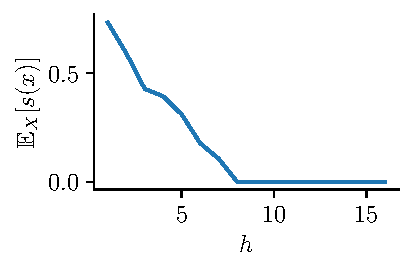
\includegraphics[scale=0.85]{data/chapter_intro/ae_reconstruction}\caption{The figure demonstrates the ability of an autoencoder to reconstruct
data. The dimensionality of the latent space $\mathcal{Z}$ is on
the x--axis, while the average reconstruction error over the whole
dataset is on the y--axis. Note that although the artificial dataset
is 16--dimensional, it only contains 8 non--correlated dimensions
while the remaining are a linear combination of them. This results
in the error dropping to zero for $\text{dim}(\mathcal{Z})>=8$ where
the model is able to disentangle the correlations and learn the identity
function.}
\label{fig:ae_reconstruction}
\par\end{centering}
\end{figure}

Suppose that $p(x)$ is the distribution of the normal data in $\mathcal{X}$
space. After training with enough examples sampled from $p(x)$, an
autoencoder should be able to reconstruct any sample from $p(x)$
almost exactly with the average error given by the constraints of
the hidden layers, as demonstrated in \ref{fig:ae_reconstruction}.
In other words, the autoencoder has learnt the shape of the distribution.
When presented with a novel sample, the ability of the autoencoder
to reconstruct it might be used to decide whether the sample comes
from $p(x)$ or not. Indeed, the most naive way of using autoencoders
for anomaly detection is assuming that $p(x)$ is the distribution
of normal data and training them using normal samples. Then, for a
novel sample $x$ the reconstruction error of the trained network
($\bar{\phi}$ and $\bar{\theta}$ are the learnt parameters of the
autoencoder)

\begin{equation}
f_{AE}(x)=\mathcal{L}_{r}(x,\bar{\phi},\bar{\theta})\label{eq:ae_score}
\end{equation}
can be used as a an anomaly score function with the assumption that
an anomaly is going to produce a larger reconstruction error due to
not coming from $p(x)$.

\subsection{Unsupervised anomaly detection}

The methods of unsupervised anomaly detection try to determine the
anomalies with no prior knowledge of the data. The dataset is evaluated
as a whole, a model of the normal class is established and the most
non-normal points are reported as anomalies. This approach assumes
that anomalies are far less frequent. Semisupervised techniques can
be adapted for the unsupervised setting when a sample of unlabeled
data is used as the training dataset, under the assumption that the
model is robust to the possible presence of contamination. Also, there
is no training dataset and the evaluation usually requires the full
dataset. One common feature of the unsupervised algorithms is that
they require an estimate of contamination rate $C(X)$ in order to
determine the threshold $\tau$.

Unsupervised anomaly detection received a great deal of attention
recently exactly because of the fact that no anomalies are needed
in advance for training of the model. Reviews of unsupervised anomaly
detection methods are presented in\,\cite{goldstein2016comparative,campos2016evaluation,chandola2009anomaly}.
Most of the unsupervised methods employ some kind of local density
estimation. One of the simplest models is the \textbf{kNN} model for
unsupervised anomaly detection where the anomaly score of a sample
is its proximity to its k--nearest samples. Several definitions of
different proximity measures are described in\,\cite{harmeling2006outliers}.
Despite its simplicity, it has been shown e.g. in\,\cite{campos2016evaluation}
that it is one of the most universal unsupervised models.

A different way of local density estimation is used in the \textbf{local
outlier factor} (LOF) algorithm\,\cite{breunig2000lof}, which is
based on comparing the local density of a sample with local densities
of its k--nearest neighbors. Similar methods are the \textbf{connectivity--based
outlier factor} (COF)\,\cite{tang2002enhancing} or \textbf{clustering--based
local outlier factor} (CBLOF)\,\cite{he2003discovering}.

A different approach is taken by the \textbf{isolation forest }(IF)
model\,\cite{liu2008isolation} where a forest of isolation trees
is constructed for the whole dataset. Isolation trees are constructed
in such a way as to isolate each individual datapoint from the rest
of the dataset using consecutive splits on different features. It
is presumed that an anomaly can be isolated using a smaller number
of splits and therefore it lies on a branch closer to the root of
the tree. The anomaly score is then the number of splits of a sample
averaged over multiple randomly initialized trees in the ensemble.

Methods based on the \textbf{PCA }transformation\,\cite{shyu2003novel,aggarwal2015outlier}\textbf{
}are also available for anomaly detection. It is presumed that normal
data lie on a lower dimensional manifold in the data space which is
extracted by selecting the covariance matrix eigenvectors with highest
corresponding eigenvalues. The distance to this manifold is then used
as anomaly score.

The \textbf{lightweight on--line detector of anomalies} (Loda)\,\cite{pevny2016loda}
algorithm is based on an ensemble of one--dimensional histograms
in a space of diversified projection vectors. The anomaly score is
then an average of the logarithm of probabilities estimated from the
histograms on individual projection vectors. Due to its simplicity
and computational efficiency, it is popular in settings with high
volumes of data and potentially missing input values.

This list is far from complete as many more models are available,
but it contains the most popular ones. As mentioned earlier, almost
any semisupervised anomaly detection model can be adopted to the unsupervised
setting. This includes the OCSVM or AE models.


